\documentclass{article}

% preamble
\def\npart{III}
\def\nyear{2019}
\def\nterm{Lent}
\def\draft{Ongoing course, rough}
\def\nlecturer{Dr T.\ Bloom}
\def\ncourse{Analytic Number Theory}

\usepackage{imakeidx}
\usepackage{chngcntr}
\usepackage[intoc, refpage]{nomencl}

\ifx \nauthor\undefined
  \def\nauthor{Bhavik Mehta}
\else
\fi

\author{Based on lectures by \nlecturer \\\small Notes taken by \nauthor}
\date{\nterm\ \nyear}
\title{Part \npart\ -- \ncourse}

\usepackage[utf8]{inputenc}
\usepackage{amsmath}
\usepackage{amsthm}
\usepackage{amssymb}
\usepackage{enumerate}
\usepackage{mathtools}
\usepackage{graphicx}
\usepackage[dvipsnames]{xcolor}
\usepackage{tikz}
\usepackage{wrapfig}
\usepackage{centernot}
\usepackage{float}
\usepackage{braket}
\usepackage[hypcap=true]{caption}
\usepackage{enumitem}
\usepackage[colorlinks=true, linkcolor=mblue]{hyperref}
\usepackage[nameinlink,noabbrev]{cleveref}
\usepackage{nameref}
\usepackage[margin=1.5in]{geometry}

% Theorems
\theoremstyle{definition}
\newtheorem*{aim}{Aim}
\newtheorem*{axiom}{Axiom}
\newtheorem*{claim}{Claim}
\newtheorem*{cor}{Corollary}
\newtheorem*{conjecture}{Conjecture}
\newtheorem*{defi}{Definition}
\newtheorem*{eg}{Example}
\newtheorem*{ex}{Exercise}
\newtheorem*{fact}{Fact}
\newtheorem*{law}{Law}
\newtheorem*{lemma}{Lemma}
\newtheorem*{notation}{Notation}
\newtheorem*{prop}{Proposition}
\newtheorem*{question}{Question}
\newtheorem*{rrule}{Rule}
\newtheorem*{thm}{Theorem}
\newtheorem*{assumption}{Assumption}

\newtheorem*{remark}{Remark}
\newtheorem*{warning}{Warning}
\newtheorem*{exercise}{Exercise}

% \newcommand{\nthmautorefname}{Theorem}

\newtheorem{nthm}{Theorem}[section]
\newtheorem{nlemma}[nthm]{Lemma}
\newtheorem{nprop}[nthm]{Proposition}
\newtheorem{ncor}[nthm]{Corollary}
\newtheorem{ndef}[nthm]{Definition}

% Special sets
\newcommand{\C}{\mathbb{C}}
\newcommand{\N}{\mathbb{N}}
\newcommand{\Q}{\mathbb{Q}}
\newcommand{\R}{\mathbb{R}}
\newcommand{\Z}{\mathbb{Z}}

\newcommand{\abs}[1]{\left\lvert #1\right\rvert}
\newcommand{\norm}[1]{\left\lVert #1\right\rVert}
\renewcommand{\vec}[1]{\boldsymbol{\mathbf{#1}}}

\let\Im\relax
\let\Re\relax

\DeclareMathOperator{\Im}{Im}
\DeclareMathOperator{\Re}{Re}
\DeclareMathOperator{\id}{id}

\definecolor{mblue}{rgb}{0., 0.05, 0.6}

\usetikzlibrary{patterns, fadings, shapes}

\makeindex[intoc]

\makenomenclature
\renewcommand{\pagedeclaration}[1]{, \hyperlink{page.#1}{#1}}
\renewcommand{\nomname}{Index of Notation}

\renewcommand{\nompreamble}{\begin{multicols}{2}}
\renewcommand{\nompostamble}{\end{multicols}}

\newcommand{\named}[1]{\textbf{#1}\index{#1}}
\newcommand{\bonusnamed}[1]{\textbf{#1}\index{#1@*#1}}
\newcommand{\bigO}{\mathcal{O}}

\DeclarePairedDelimiter\floor{\lfloor}{\rfloor}
\DeclarePairedDelimiter\ceil{\lceil}{\rceil}

\setcounter{section}{-1}
% \counterwithout{nthm}{section}

% and here we go!
\begin{document}
\maketitle

\tableofcontents

\clearpage
\section{Introduction}
\newlec
Analytic Number Theory is the study of numbers using analysis. It is a fascinating field because because a number - in particular in this course an integer - is discrete, whilst analysis involves the real/complex numbers which are continuous.

In this course, we will ask quantitative questions things like `how many' or `how large', in reference to simple number-theoretic objects.

\begin{eg}\leavevmode
  \begin{enumerate}
    \item How many primes? We can define the \index{prime-counting function}prime-counting function\nomenclature{$\pi(x)$}{prime-counting function}
      \begin{equation*}\hypertarget{def:pi}\pi(x) = |\{n : n \leq x \text{ and } n \text{ is prime} \}|.\end{equation*}
      Then the \hypertarget{def:pntold}prime number theorem\index{prime number theorem}, which we will prove in this course, states
      \begin{equation*}\pi(x) \sim \frac{x}{\log x}.\end{equation*}
      (We will always take `numbers' to mean natural numbers, not including zero).
    \item How many twin primes ($p$ such that $p+2$ is also prime) are there?
      It is not known whether there are infinitely many but since 2014, there has been immense progress by Zhang, Maynard and a Polymath project which has determined there are infinitely many primes at most 246 apart.
      Guess: there are $\approx \frac{x}{(\log x)^2}$ many twin primes $\leq x$.
    \item How many primes are there congruent to $a \bmod q$ where $(a,q) = 1$. We know, by Dirichlet's theorem proven in the 20th century, that there are infinitely many such.
      The guess for how many there are in the interval $[1,x]$ is
      \begin{equation*}
        \frac{1}{\varphi(q)} \frac{x}{\log x}.
      \end{equation*}
      This is known for small $q$. Recall that $\varphi(n) \coloneqq |\{1\leq m \leq n : (m,n) =1 \}|$, Euler's totient function.\index{totient function}\nomenclature{$\varphi(x)$}{Euler's totient function}
  \end{enumerate}
\end{eg}
The course will be split up into 4 (roughly equal) parts
\begin{enumerate}
  \item Elementary techniques (real analysis)
  \item Sieve methods
  \item Riemann Zeta function, Prime Number Theorem (complex analysis)
  \item Primes in arithmetic progressions
\end{enumerate}
\clearpage

\section{Elementary Techniques}
We begin with a review of asymptotic notations:
\begin{itemize}\hypertarget{def:asymp}
  \item \nomenclature{$\bigO$}{Big $\bigO$ notation; Landau notation}$f(x) = \bigO(g(x))$ if there is $C>0$ such that $|f(x)| \leq C|g(x)|$ for all large enough $x$. (Landau notation)
  \item \nomenclature{$\ll$}{Vinogradov notation}$f \ll g$ is the same as $f = \bigO(g)$ (Vinogradov notation)
  \item \nomenclature{$\sim$}{asymptotic equality}$f\sim g$ if $\lim_{x \to \infty}\frac{f(x)}{g(x)} = 1 $ (i.e.\ $f = (1+o(1))g$).
  \item \nomenclature{$o$}{Little $o$ notation}$f= o(g)$ if $\lim_{x \to \infty}\frac{f(x)}{g(x)} = 0$
\end{itemize}

\subsection{Arithmetic Functions}
\begin{defi}\hypertarget{def:arith}
  An \named{arithmetic function} is a function $f : \mathbb{N} \to \mathbb{C}$.
\end{defi}
\begin{defi}\hypertarget{def:conv}
  An important operation for multiplicative number theory is the \textbf{multiplicative convolution\index{convolution}}
  \nomenclature{$\star$}{convolution}
  \begin{equation*}f\star g(n) \coloneqq \sum_{ab = n} f(a)g(b).\end{equation*}
\end{defi}
\begin{eg}\leavevmode
  \begin{itemize}
    \item \hypertarget{def:1}{$1(n) \coloneqq 1 \; \; \forall n$}\nomenclature{$1(n)$}{constant 1 function}. Caution: $1\hyperlink{def:conv}{\star} f \neq f$.
    \item \hypertarget{def:mu}M\"obius function:\index{M\"obius function}\nomenclature{$\mu(n)$}{M\"obius function}
      \begin{equation*}
        \mu(n) =
        \begin{cases*}
          (-1)^k & if $n = p_1\dotsm p_k$ \\
          0 & if $n$ not squarefree
        \end{cases*}
      \end{equation*}
    \item \hypertarget{def:lamb}Liouville function:\index{Liouville function}\nomenclature{$\lambda(n)$}{Liouville function}
      \begin{equation*}
        \lambda(n) = (-1)^k \text{ if } n = p_1\dotsm p_k, \text{ not necessarily distinct}
      \end{equation*}
    \item \hypertarget{def:tau}Divisor function:\index{divisor function}\nomenclature{$\tau$}{divisor function}
      \begin{align*}
        \tau(n) &= | \{ d \mid d\text{ a factor of }n \} | \\
        \tau &= \hyperlink{def:1}{1} \hyperlink{def:conv}{\star}1
      \end{align*}
  \end{itemize}
\end{eg}
\begin{defi}[Multiplicative function]\hypertarget{def:multi}
  An \hyperlink{def:arith}{arithmetic function} is a \named{multiplicative function} if $f(nm) = f(n)f(m)$ for $(n,m) =1$.
  In particular, a multiplicative function is determined by its values on prime powers $f(p^k)$.
\end{defi}
\begin{fact}\leavevmode
  \begin{itemize}
    \item If $f,g$ are \hyperlink{def:multi}{multiplicative}, then so is $\hyperlink{def:conv}{f\star g}$.
    \item $\log n $ is not multiplicative.
      $1,\mu,\lambda,\tau$ are multiplicative.
  \end{itemize}
  Note almost all \hyperlink{def:arith}{arithmetic functions} are not multiplicative.
\end{fact}
\begin{fact}[\hypertarget{def:mobinv}M\"obius inversion]\index{M\"obius function}
  \begin{equation*}
    \hyperlink{def:1}{1} \hyperlink{def:conv}{\star} f = g \iff \hyperlink{def:mu}{\mu} \star g = f.
  \end{equation*}
\end{fact}

\begin{proof}
  First show
  \begin{equation*}
    1 \hyperlink{def:star}{\star} \hyperlink{def:mu}{\mu}(n) \coloneqq
    \sum_{d \mid n} \hyperlink{def:mu}{\mu(d)} =
    \begin{cases*}
      1 & if $n=1$ \\
      0 & otherwise.
    \end{cases*}
  \end{equation*}
  We have $1,\mu$ are \hyperlink{def:multi}{multiplicative}, so $1\star\mu$ is multiplicative.
  Hence it is enough to check the identity for prime powers:
  If $n= p^k$, then $\{d : d\text{ divides }n\} = \{1,p,\ldots,p^k\}$ so the left hand side is $1-1 + 0 + \ldots + 0 = 0$, unless $k=0$ when the left hand side is $\mu(1) =1$.

  The right hand side here is the identity of \hyperlink{def:conv}{convolution}, and convolution is associative, giving the required result.
\end{proof}

Our ultimate goal is to study the primes. This would suggest that we should work with the indicator function of the primes:
\begin{equation*}
  1_p(n) = \begin{cases*}
    1 &if $n$ prime \\
    0 & otherwise.
  \end{cases*}
\end{equation*}
For example $\pi(x) = \displaystyle \sum_{\mathclap{1\leq n\leq x}} 1_p(n)$.
This is an awkward function to work with.
Instead, define the \nomenclature{$\Lambda(n)$}{von Mangoldt function}\named{von Mangoldt function}
\begin{equation*}
  \hypertarget{def:vonMang}\Lambda(n) =
  \begin{cases*}
    \log p & if $n$ is a prime power\\
    0 & otherwise
  \end{cases*}
\end{equation*}
i.e.\ weight the prime powers.
This function is easier to use. Why?
\begin{lemma}
  \begin{equation*}
    \hyperlink{def:1}{1} \hyperlink{def:conv}{\star} \hyperlink{def:vonMang}{\Lambda} = \log \quad \text{and} \quad \hyperlink{def:mu}{\mu} \star \log = \Lambda
  \end{equation*}
\end{lemma}
\begin{proof}
  The second part follows immediately by \hyperlink{def:mobinv}{M\"obius inversion} from the first.
  \begin{align*}
    1\star \hyperlink{def:vonMang}{\Lambda(n)} & = \sum_{d \mid n}\Lambda(d)\\
    \shortintertext{so write $n = p_1^{k_1}\ldots p_k^{n_k}$,}
                 &= \sum_{i=1}^r \sum_{j=1}^{k_i} \Lambda(p_i^j) \\
                 &= \sum_{i=1}^r \sum_{j=1}^{k_i} \log p_i \\
                 &= \sum_{i=1}^{r}k_i\log p_i
                 = \sum_{i=1}^{r}\log p_i^{k_i}
                 = \log n. \qedhere
  \end{align*}
\end{proof}
\begin{eg}
  We can write
  \begin{align*}
    \hyperlink{def:vonMang}{\Lambda(n)} &= \sum_{d|n}\hyperlink{def:mu}{\mu(d)}\log\left(\frac{n}{d}\right) \\
                                        &= \log n \sum_{d|n}\mu(d) - \sum_{d|n}\mu(d)\log d \\
                                        &= - \sum_{d|n}\mu(d)\log d.
  \end{align*}

  \begin{align*}
    \sum_{\mathclap{1\leq n \leq x}}{\Lambda(n)} &= -\sum_{1\leq n\leq x}\sum_{d|n}{\mu(d)}\log d \\
                                    &= - \sum_{d\leq x}\mu(d)\log(d)\Big(\sum_{\substack{1\leq n\leq x \\ d|n}}1\Big)
                                    \shortintertext{but $\sum_{\substack{1\leq n\leq x \\ d|n}}1 = \floor*{\frac{x}{d}}= \frac{x}{d} + \bigO(1)$, so}
                                    &= - x \sum_{d\leq x}\mu(d) \frac{\log d}{d} + \hyperlink{def:asymp}{\bigO}\bigg(\sum_{d\leq x}\mu(d)\log d \bigg). \qedhere
  \end{align*}
\end{eg}
\clearpage

\subsection{Partial summation}
\newlec
Given an \hyperlink{def:arith}{arithmetic function}, we can ask for estimates of $\sum_{n \leq x} f(n)$, which gives a rough idea of how large $f(n)$ is on average.
\begin{defi}\hypertarget{def:averageOrder}
We say that $f$ has \named{average order} $g$ if
\begin{equation*}\sum_{1 \leq n \leq x} f(n) \hyperlink{def:asymp}{\sim} x g(x).\end{equation*}
\end{defi}
\begin{eg}
  For example, if $f \equiv 1$,
  \begin{equation*}
    \sum_{1 \leq n \leq x} f(n) = \floor{x} = x + \hyperlink{def:asymp}{\bigO}(1) \sim x
  \end{equation*}
  so \hyperlink{def:averageOrder}{average order} of $f$ is $1$.
  Now take $f(n) = n$,
  \begin{equation*}
    \sum_{1 \leq n \leq x} n \sim \frac{x^2}{2}
  \end{equation*}
  so the average order of $n$ is $\frac{n}{2}$.
  The \hyperlink{def:pntold}{Prime Number Theorem} is the statement that $1_p$ has average order $\frac{1}{\log x}$.
\end{eg}

\begin{nlemma}[Partial summation]\label{lem:1}
  If $(a_n)$ is a sequence of complex numbers and $f$ is such that $f'$ is continuous, then
  \begin{equation*}
    \sum_{1 \leq n \leq x} a_n f(n) = A(x) f(x) - \int_1^x A(t) f'(t) \, dt
  \end{equation*}
  where $A(x) = \sum_{1 \leq n \leq x} a_n$.
\end{nlemma}

\begin{proof}
  Suppose $x = N$ is an integer. Note that $a_n = A(n) - A(n-1)$.
  So
  \begin{align*}
    \sum_{1 \leq n \leq N} a_n f(n) &= \sum_{1 \leq n \leq N} f(n) \left(A(n) - A(n-1)\right) \\
    \shortintertext{(note $A(0) = 0$)}
    &= A(N) f(N) + \sum_{n=1}^{N-1} A(n) \left(f(n+1)-f(n)\right).
  \end{align*}
  Now
  \begin{align*}f(n+1)-f(n) = \int_{n}^{n+1}\!\!f'(t)\,dt.\end{align*}
  So
  \begin{align*}
    \sum_{1 \leq n \leq N} a_n f(n) &= A(N) f(N) - \sum_{n=1}^{N-1} f'(t) \, dt \\
                                    &= A(N) f(N) - \int_1^N A(t) f'(t) \, dt
  \end{align*}
  where we set $A(n) = A(t) \; \forall t \in [n, n+1)$. %]
  If $N > \floor{x}$, i.e.\ $x$ not an integer,
  \begin{align*}
    A(x) f(x) &= A(N) f(x) \\
              &= A(N) \left(f(N) + \int_N^x f'(t) \, dt\right). \qedhere
  \end{align*}
\end{proof}
\begin{nlemma}\label{lem:2}
  \begin{align*}
    \sum_{1 \leq n \leq x} \frac{1}{n} = \log x + \gamma + \hyperlink{def:asymp}{\bigO}\left(\tfrac{1}{x}\right)
  \end{align*}
\end{nlemma}
\begin{proof}
  \nameref{lem:1} with $f(x) = \frac{1}{x}$ and $a_n = 1$, so $A(x) = \floor{x}$:
  \begin{align*}
    \sum_{1 \leq n \leq x} \frac{1}{n} &= \frac{\floor{x}}{x} + \int_1^x \frac{\floor{t}}{t^2}\,dt \\
    \shortintertext{recall $\floor{t} = t - \{t\}$}
                                       &= 1 + \hyperlink{def:asymp}{\bigO}\left(\tfrac{1}{x}\right) + \int_1^x \frac{1}{t}\,dt - \int_1^x \frac{\{t\}}{t^2}\,dt \\
                                       &= 1 + \bigO\left(\tfrac{1}{x}\right) + \log x -\int_1^\infty \frac{\{t\}}{t^2} \, dt + \underbrace{\int_x^\infty \frac{\{t\}}{t^2}\,dt}_{\leq \int_x^\infty \frac{1}{t^2}\,dt \leq \frac{1}{x}} \\
                                       &=\gamma + \bigO\left(\tfrac{1}{x}\right) + \log x + \bigO\left(\tfrac{1}{x}\right) \\
                                       &= \log x + \gamma + \bigO\left(\tfrac{1}{x}\right)
  \end{align*}
  where $\gamma = 1 - \int_1^\infty \frac{\{t\}}{t^2} \, dt$.
\end{proof}
\hypertarget{def:gamma}This $\gamma$ is called Euler's constant (Euler-Mascheroni). $\gamma \approx 0.577\dots$ but we don't know if $\gamma$ is irrational or not.

\begin{nlemma}\label{lem:3}
  \begin{equation*}
    \sum_{\mathclap{1 \leq n \leq x}}\ \log n = x \log x - x + \hyperlink{def:asymp}{\bigO}(\log x).
  \end{equation*}
\end{nlemma}
\begin{proof}
  \nameref{lem:1} with $f(x) = \log x$, $a_n = 1$, $A(x) = \floor{x}$.
  \begin{align*}
    \sum_{\mathclap{1 \leq n \leq x}}\ \log n &= \floor{x} \log x - \int_1^x \frac{\floor{t}}{t} \, dt \\
                                  &= x \log x + \hyperlink{def:asymp}{\bigO}(\log x) - \int_1^x 1 \, dt + \bigO\left(\int_1^x \frac{1}{t} \, dt\right) \\
                                  &= x \log x + \bigO(\log x) - x + \bigO(\log x) \\
                                  &= x \log x - x + \bigO(\log x). \qedhere
  \end{align*}
\end{proof}
This is not really Number Theory - we haven't really used multiplication yet.
\subsection{Divisor function}
Recall that
\begin{equation*}
\hyperlink{def:tau}{\tau(n)} = \hyperlink{def:1}{1} \hyperlink{def:conv}{\star} 1 (n) = \sum_{ab \mid n} 1 = \sum_{d \mid n} 1
\end{equation*}
We will analyse how many divisors an integer has.
\begin{nthm}\label{thm:4}
  \begin{align*}
    \sum_{\mathclap{1 \leq n \leq x}} \hyperlink{def:tau}{\tau(n)} = x \log x + (2 \gamma - 1) x + \hyperlink{def:asymp}{\bigO}(x^{\frac{1}{2}})
  \end{align*}
  So \hyperlink{def:averageOrder}{average order} of $\tau$ is $\log x$.
\end{nthm}
\begin{proof}
  \nameref{lem:1} involves turning a sum $\sum a_n \rightsquigarrow \sum a_n f(n)$, but what does $\hyperlink{def:tau}{\tau(\frac{1}{2})}$ even mean?
  There is no continuous function to use.

  Instead, play around with the definition:
  \begin{align*}
    \sum_{\mathclap{1 \leq n \leq x}} \tau(n) &= \sum_{1 \leq n \leq x} \sum_{d \mid x} 1 \\
                                   &= \sum_{1 \leq d \leq x} \sum_{\substack{1 \leq n \leq x \\ d \mid n}} 1
                                   \shortintertext{note that $\sum_{\substack{1 \leq n \leq x \\ d \mid n}} 1 = \floor{\frac{x}{d}}$}
                                   &= \sum_{1 \leq d \leq x} \floor*{\frac{x}{d}} \\
                                   &= \sum_{1 \leq d \leq x} \frac{x}{d} + \hyperlink{def:asymp}{\bigO}(x) \\
                                   &= x \sum_{1 \leq d \leq x} \frac{1}{d} + \bigO(x) \\
                                   &= x \log x + \gamma x + \bigO(x)
  \end{align*}
  using \cref{lem:2}.
  To reduce the error term, we use (Dirichlet's) hyperbola trick.
  \begin{equation*}
    \sum \tau(n) = \sum_{1 \leq n \leq x} \sum_{a b = n} 1 = \sum_{ab \leq x} 1 = \sum_{a \leq x} \sum_{b \leq \frac xa} 1
  \end{equation*}
  \begin{tikzfadingfrompicture}[name=edge fade]
    \fill [white] (0,0) rectangle (4,4);
    \shade [left color=white, right color=transparent!100] (4,0) rectangle (5,4);
    \shade [bottom color=white, top color=transparent!100] (0,4) rectangle (4,5);
    \fill [transparent] (4,4) rectangle (5,5);
  \end{tikzfadingfrompicture}
  \begin{center}
    \begin{tikzpicture}
      \draw [<->] (5.2,0) -- (0,0) -- (0,5.2);
      \draw [very thin] (2,0) -- (2,2) -- (0,2);
      \begin{scope}
        \path [scope fading=edge fade, fit fading=false, fading transform={shift={(2.5,2.5)}}] (0,0) rectangle (5,5);
        \draw [domain=0.4:2.5,scale=2,smooth,variable=\x] plot ({\x},{1/\x});
        \fill [opacity=0.7, pattern=north east lines, pattern color=bred!70!black] [domain=1:2.5,scale=2,smooth,variable=\x] plot ({\x},{1/\x}) -- (2.5,0) -- (0,0) -- (0,1) -- (1,1);
        \fill [opacity=0.7, pattern=north west lines, pattern color=bblue!70!black] [domain=0.4:1,scale=2,smooth,variable=\x] plot ({\x},{1/\x}) -- (1,0) -- (0,0) -- (0,2.5) -- (0.4,2.5);
      \end{scope}
    \end{tikzpicture}
  \end{center}
  When summing over $ab \leq x$, we can sum over $a \leq x^{\frac{1}{2}}$, $b \leq x^{\frac{1}{2}}$ separately, and subtract the overlap.
  \begin{align*}
    \sum_{1 \leq n \leq x} \tau(n) &= \sum_{a \leq x^{\frac{1}{2}}} \sum_{b \leq \frac{x}{a}} 1 + \sum_{b \leq x^{\frac{1}{2}}} \sum_{a \leq \frac{x}{b}} 1 - \sum_{\mathclap{a,b \leq x^{\frac{1}{2}}}} 1 \\
                                   &= 2 \sum_{a \leq x^{\frac{1}{2}}} \floor*{\frac{x}{a}} - \underbrace{\floor*{x^{\frac{1}{2}}}^2}_{\mathclap{=\left(x^{\frac{1}{2}} + \bigO(1)\right)^2}} \\
                                   &= 2 \sum_{a \leq x^{\frac{1}{2}}} \frac{x}{a} + \bigO(x^{\frac{1}{2}}) - x + \bigO(x^{\frac{1}{2}}) \\
                                   &= 2 x \log x^{\frac{1}{2}} + 2 \gamma x - x + \bigO(x^{\frac{1}{2}}) \\
                                   &= x \log x + (2 \gamma - 1) x + \bigO(x^{\frac{1}{2}}). \qedhere
  \end{align*}
\end{proof}
Analytic Number Theory is mostly just controlling the error term.
\begin{remark}
  Improving this $\bigO(x^{\frac{1}{2}})$ error term is a famous and hard problem! Probably, $\bigO(x^{\frac{1}{4} + \epsilon})$. The current best known is $\bigO(x^{0.3148})$.

  This does not mean that $\tau(n) = \log n$: the average order does not give any information about specific values.
\end{remark}
\begin{nthm}\label{thm:5}
  \newlec
  For any $n \geq 1$,
  \begin{equation*}
    \hyperlink{def:tau}{\tau(n)} \leq n^{\hyperlink{def:asymp}{\bigO}\left(\frac{1}{\log \log n}\right)}.
  \end{equation*}
  In particular,
  \begin{equation*}
    \tau(n) \ll_\epsilon n^\epsilon \; \forall \epsilon > 0
  \end{equation*}
  i.e.\ $\forall \epsilon > 0$, $\exists C(\epsilon) > 0$ such that $\tau(n) \leq C n^\epsilon$.
\end{nthm}
\begin{proof}
  \hyperlink{def:tau}{$\tau$} is \hyperlink{def:multi}{multiplicative}, so enough to calculate at prime powers. $\tau(p^k) = k+1$, so if $n = p_1^{k_1} \dotsm p_r^{k_r}$ then
  \begin{equation*}
    \tau(n) = \prod_{i=1}^r (k_i + 1).
  \end{equation*}
  Let $\epsilon > 0$ be chosen later and consider $\frac{\tau(n)}{n^\epsilon}$.
  \begin{equation*}
    \frac{\tau(n)}{n^\epsilon} = \prod_{i=1}^r \frac{k_i+1}{p^{k_i \epsilon}}.
  \end{equation*}
  Note that as $p$ is large, $\frac{k+1}{p^{k\epsilon}} \to 0$. In particular, if $p \geq 2^{\frac{1}{\epsilon}}$, then $\frac{k+1}{p^{k\epsilon}} \leq \frac{k+1}{2^k} \leq 1$.

  What about small $p$? Can't do better than $p \geq 2$.
  In this case, $\frac{k+1}{p^{k\epsilon}} \leq \frac{k+1}{2^{k\epsilon}} \leq \frac{1}{\epsilon}$.
  Why? Rearrange to say $\epsilon k + \epsilon \leq 2^{k \epsilon}$ (if $\epsilon \leq \frac{1}{2}$), which follows from $x + \frac{1}{2} \leq 2^x \; \forall x \geq 0$

  So
  \begin{equation*}
    \frac{\tau(n)}{n^\epsilon} \leq \prod_{\substack{i=1 \\ p_i < 2^{\frac{1}{\epsilon}}}} \frac{k_i + 1}{p^{k_i \epsilon}} \leq \left(\frac{1}{\epsilon}\right)^{\pi(2^{\frac{1}{\epsilon}})} \leq \left(\frac{1}{\epsilon}\right)^{2^{\frac{1}{\epsilon}}}.
  \end{equation*}

  Now choose optimal $\epsilon$.
  (Trick: if you want to choose $x$ to minimise $f(x) + g(x)$, choose $x$ such that $f(x) = g(x)$).

  So have,
  \begin{equation*}
    \tau(n) \leq n^\epsilon \epsilon^{-2^{\frac{1}{\epsilon}}} = \exp\left(\epsilon \log n + 2^{\frac{1}{\epsilon}} \log \frac{1}{\epsilon}\right).
  \end{equation*}
  Choose $\epsilon$ such that $\log n \approx 2^{\frac{1}{\epsilon}}$, i.e.\ $\epsilon \approx \frac{1}{\log \log n}$.
  \begin{equation*}
    \tau(n) \leq n^{\frac{1}{\log \log n}} (\log \log n)^{2^{\log \log n}} = n^{\frac{1}{\log \log n}} e^{(\log n)^{\log 2} \log \log \log n} \leq n^{\bigO(\frac{1}{\log \log n})}. \qedhere
  \end{equation*}
\end{proof}
\subsection{Estimates for the primes}
Recall
\begin{align*}
  \pi(x) &= \abs{\set{p \leq x}} = \sum_{\mathclap{1\leq n \leq x}} 1_p(n)
  \shortintertext{and}
  \nomenclature{$\psi(x)$}{summatory von Mangoldt function}\hypertarget{def:psi}\psi(x) &= \sum_{1 \leq n \leq x} \hyperlink{def:vonMang}{\Lambda(n)}.
\end{align*}
\hypertarget{def:pnt}The Prime Number Theorem is $\pi(x) \hyperlink{def:asymp}{\sim} \frac{x}{\log x}$ or equivalently $\psi(x) \sim x$.
It was 1850 before the correct magnitude of $\pi(x)$ was proved.
Chebyshev showed $\pi(x) \asymp \frac{x}{\log x}$, (\hypertarget{def:asymp2}where $f \asymp g$ means $g \hyperlink{def:asymp}{\ll} f \ll g$).

\begin{nthm}[Chebyshev]\label{thm:6}
  \begin{equation*}
    \hyperlink{def:psi}{\psi(x)} \hyperlink{def:asymp2}{\asymp} x
  \end{equation*}
\end{nthm}
\begin{proof}
  First we'll prove the lower bound, i.e.\ that $\hyperlink{def:psi}{\psi(x)} \hyperlink{def:asymp}{\gg} x$.
  \begin{equation*}
    \psi(x) = \sum_{n \leq x} \hyperlink{def:vonMang}{\Lambda(n)}.
  \end{equation*}
  $x \log x$ is a trivial upper bound for this, (each summand is $\leq \log x$); we'd like to remove the factor of $\log x$.
  Recall $1 \hyperlink{def:conv}{\star} \Lambda = \log$, i.e.\
  \begin{equation*}\sum_{ab=n} \Lambda(a) = \log n.\end{equation*}
  The trick is to find a sum $\Sigma$ such that $\Sigma \leq 1$.
  We'll use the identity $\floor{x} \leq 2 \floor{\frac{x}{2}} + 1$, valid for $x \geq 0$.
  (Proof: Say $\frac{x}{2} = n + \theta$, with $\theta \in [0,1)$, so $\floor{\frac{x}{2}} = n$ then $x = 2n + 2\theta$ so $\floor{x} = 2n$ or $2n+1$.)

  So
  \begin{align*}
    \psi(x) &\geq \sum_{n \leq x} \Lambda(n) \left(\floor{\tfrac{x}{n}} - 2 \floor{\tfrac{x}{2n}}\right). \\
    \shortintertext{Note $\floor{\frac{x}{n}} = \sum_{m \leq \frac{x}{n}} 1$}.
            &= \sum_{n \leq x} \Lambda(n) \sum_{m \leq \frac xn} 1 - 2 \sum_{n \leq x} \Lambda(n) \sum_{m \leq \frac x {2n}} 1 \\
            &= \sum_{mn \leq x} \Lambda(n) - 2 \sum_{\mathclap{nm \leq \frac x2}} \Lambda(n) \\
            &= \sum_{d \leq x} 1 \star \Lambda(d) - 2 \sum_{d \leq \frac x2} 1 \star \Lambda(d) \\
            &= \sum_{d \leq x} \log d - 2 \sum_{d \leq \frac{x}{2}} \log d \\
            &= x \log x - x + \hyperlink{def:asymp}{\bigO}(\log x) - 2 \left(\frac{x}{2} \log \frac{x}{2} - \frac{x}{2} + \bigO(\log x)\right) \\
            &= (\log 2) x + \bigO(\log x) \gg x.
  \end{align*}

  For the upper bound, note $\floor{x} = 2 \floor{\frac{x}{2}} + 1$ for $x \in (1,2)$ so
  \begin{equation*}
    \sum_{\mathclap{\frac{x}{2} < n < x}} \Lambda(n) = \sum_{\mathclap{\frac{x}{2} < n < x}} \Lambda(n) \left(\floor{\tfrac{x}{n}} - 2 \floor{\tfrac{x}{2n}}\right) \leq \sum_{\mathclap{1 \leq n \leq x}} \Lambda(n) \left(\floor{\tfrac{x}{n}} - 2 \floor{\tfrac{x}{2n}}\right)
  \end{equation*}
  Thus
  \begin{align*}
    \psi(x) - \psi\left(\frac{x}{2}\right) &\leq (\log 2) x + \bigO(\log x). \\
    \psi(x) &= \left(\psi(x) - \psi\left(\tfrac{x}{2}\right)\right) + \left(\psi(\tfrac{x}{2}) - \psi(\tfrac{x}{4})\right) + \dotsb  \\
            &\leq \log 2\left(x + \tfrac{x}{2} + \tfrac{x}{4} + \dotsb\right) + \bigO((\log x)^2)\\
    &= 2 \log 2 x + \bigO((\log x)^2). \qedhere
  \end{align*}
\end{proof}
\begin{nlemma}\label{lem:7}
  \begin{equation*}
    \sum_{p \leq x} \frac{\log p}{p} = \log x + \hyperlink{def:asymp}{\bigO}(1).
  \end{equation*}
\end{nlemma}
\begin{proof}
  Recall $\log = 1 \hyperlink{def:conv}{\star} \hyperlink{def:vonMang}{\Lambda}$. So
  \begin{align*}
    \sum_{n \leq x} \log n &= \sum_{ab \leq x} \Lambda(a) = \sum_{a \leq x} \Lambda(a) \sum_{b \leq \frac{x}{a}} 1 \\
                           &= \sum_{a \leq x} \Lambda(a) \floor{\tfrac{x}{a}} = x \sum_{a \leq x} \frac{\Lambda(a)}{a} + \hyperlink{def:asymp}{\bigO}(\hyperlink{def:psi}{\psi(x)}) \\
                           &= x \sum_{a \leq x} \frac{\Lambda(a)}{a} + \bigO(x) \\
  \shortintertext{But from \cref{lem:3},}
    \sum_{n \leq x} \log n &= x \log x - x + \bigO(\log x) \\
    \text{So }\sum_{n \leq x} \frac{\Lambda(n)}{n} &= \log x - 1 + \mathcal{O}(\tfrac{\log x}{x}) + \bigO(1) = \log x + \bigO(1).
  \end{align*}

  Remains to note
  \begin{align*}
    \sum_{p \leq x} \sum_{n=2}^\infty \frac{\log p}{p^k} = \sum_{p \leq x} \log p \sum_{k=2}^\infty \frac{1}{p^k} = \sum_{p \leq x} \frac{\log p}{p^2 - p} \leq \sum_{p=2}^\infty \frac{1}{p^{\frac{3}{2}}} = \bigO(1).
  \end{align*}
  So
  \begin{equation*}\sum_{n \leq x} \frac{\Lambda(n)}n = \sum_{p \leq x} \frac{\log p}{p} + \bigO(1).\qedhere\end{equation*}
\end{proof}
\begin{nlemma}\label{lem:8}
  \newlec
  \begin{equation*}
    \hyperlink{def:pi}{\pi(x)} = \frac{\hyperlink{def:psi}{\psi(x)}}{\log x} + \hyperlink{def:asymp}{\bigO}\left(\frac{x}{(\log x)^2}\right).
  \end{equation*}
\end{nlemma}
In particular, $\pi(x) \hyperlink{def:asymp2}{\asymp} \frac{x}{\log x}$ and the statement of the prime number theorem ($\pi(x) \hyperlink{def:asymp}{\sim} \frac{x}{\log x}$) is equivalent to $\psi(x) \sim x$.
\begin{proof}
  Idea is to use \nameref{lem:1}:
  \begin{equation*}
    \theta(x) \coloneqq \sum_{p \leq x} \log p = \hyperlink{def:pi}{\pi(x)} \log x - \int_1^x \frac{\pi(t)}{t} \, dt
  \end{equation*}
  whereas
  \begin{equation*}\hyperlink{def:psi}{\psi(x)} = \sum_{n \leq x} \hyperlink{def:vonMang}{\Lambda(n)} = \sum_{p^k \leq x} \log p.\end{equation*}
  \begin{align*}
    \psi(x) - \theta(x) = \sum_{k=2}^\infty \sum_{p^k \leq x} \log p = \sum_{k=2}^\infty \theta(x^{\frac{1}{k}}) \leq \sum_{k=2}^{\log x} \psi(x^{\frac{1}{k}}) \ll \sum_{k=2}^{\log x} x^{\frac{1}{k}} \ll x^{\frac{1}{2}} \log x
  \end{align*}
  Thus,
  \begin{align*}
    \psi(x) &= \pi(x) \log x + \hyperlink{def:asymp}{\bigO}(x^{\frac{1}{2}} \log x) - \int_1^x \frac{\pi(t)}{t} \, dt \\
            &= \pi(x) \log x + \bigO(x^{\frac{1}{2}}) + \bigO\left(\int_1^x \frac{1}{\log t} \, dt\right) \\
            &= \pi(x) \log x + \bigO\left(\frac{x}{\log x}\right)
  \end{align*}
  where we used the fact that $\pi(t) \ll \frac{t}{\log t}$:
  Trivially, $\pi(t) \leq t$, so
  \begin{equation*}
    \psi(x) = \pi(x) \log x + \bigO(x^{\frac{1}{2}} \log x) + \bigO(x)
  \end{equation*}
  so $\pi(x) \log x = \bigO(x)$.
\end{proof}
\begin{nlemma}\label{lem:9}
  \begin{equation*}
    \sum_{p \leq x} \frac{1}{p} = \log \log x + b + \hyperlink{def:asymp}{\bigO}(\tfrac{1}{\log x})
  \end{equation*}
  where $b$ is some constant.
\end{nlemma}
\begin{proof}
  We use partial summation. Let $A(x) = \sum_{p \leq x} \frac{\log p}{p} = \log x + R(x)$ (and $R(x) \hyperlink{def:asymp}{\ll} 1$).
  \begin{align*}
    \sum_{2 \leq p\leq x} \frac{1}{p} &= \frac{A(x)}{\log x} + \int_2^x \frac{A(t)}{t (\log t)^2} \, dt \\
    &= 1 + \hyperlink{def:asymp}{\bigO}(\tfrac{1}{\log x}) + \int_2^x \frac{1}{t \log t} \, dt + \int_2^x \frac{R(t)}{t (\log t)^2} \, dt
  \end{align*}
  Note $\int_2^\infty \frac{R(t)}{t (\log t)^2} \, dt$ exists, say it is $c$.
  \begin{align*}
    \sum_{2 \leq p \leq x} \frac{1}{p} &= 1 + c + \bigO(\tfrac{1}{\log x}) + \log \log x - \log \log 2 + \bigO\left(\int_x^\infty \frac{1}{t (\log t)^2}\right) \\
                                       &= \log \log x + b + \bigO\left(\tfrac{1}{\log x}\right). \qedhere
  \end{align*}
\end{proof}
\begin{nthm}[Chebyshev]\label{thm:10}
  If
  \begin{equation*}
    \hyperlink{def:pi}{\pi(x)} \sim c \frac{x}{\log x}
  \end{equation*}
  then $c = 1$.
\end{nthm}
Chebyshev also showed if $\pi(x) \sim \frac{x}{\log x - A(x)}$ then $A \sim 1$, which was a surprise since it was believed $A \sim 1.08\dots$
\begin{proof}
  \nameref{lem:1} on $\sum_{p \leq x} \frac{1}{p}$.
  \begin{align*}
    \sum_{p \leq x} \frac{1}{p} &= \frac{\pi(x)}{x} + \int_1^x \frac{\pi(t)}{t^2} \, dt.
    \shortintertext{If $\pi(x) = (c + o(1)) \frac{x}{\log x}$ then }
                    &= \frac{c}{\log x} + o\left(\frac{1}{\log x}\right) + (c + o(1)) \int_1^x \frac{1}{t \log t} \, dt \\
                    &= \bigO\left(\frac{1}{\log x}\right) + (c+o(1)) \log \log x.
  \end{align*}
  But $\sum_{p \leq x} \frac{1}{p} = (1 + o(1)) \log \log x$ by \cref{lem:9}. Hence $c = 1$.
\end{proof}
\begin{nlemma}\label{lem:11}
  \begin{equation*}
    \prod_{p \leq x} \left(1 - \frac{1}{p}\right)^{-1} = c \log x + \hyperlink{def:asymp}{\bigO}(1)
  \end{equation*}
  where $c$ is some constant.
\end{nlemma}
\begin{proof}
  \begin{align*}
    \log \left(\prod_{p \leq x} \left(1 - \frac{1}{p}\right)^{-1}\right) &= - \sum_{p \leq x} \log \left(1 - \frac{1}{p}\right) \\
                                                                         &= \sum_{p \leq x} \sum_{k} \frac{1}{k p^k} \\
                                                                         &= \sum_{p \leq x} \frac 1p + \sum_{k \geq 2} \sum_{p \leq x} \frac{1}{k p^k} \\
                                                                         &= \log \log x + c' + \hyperlink{def:asymp}{\bigO}\left(\frac{1}{\log x}\right).
  \end{align*}
  Now note that $e^x = 1 + \bigO(x)$ for $|x| \leq 1$.
  So
  \begin{align*}
    \prod_{p \leq x} \left(1 - \frac{1}{p}\right)^{-1} = c \log x\ e^{\bigO(\frac{1}{\log x})} &= c \log x\ (1 + \bigO(\tfrac{1}{\log x})) \\
                                                                                            &= c \log x + \bigO(1). \qedhere
  \end{align*}
\end{proof}
It turns out that $c = e^\gamma = 1.78\dots$

\subsubsection{Why is the Prime Number Theorem hard?}
Let's try a probabilistic heuristic for the PNT: the `probability' that $p \mid n$ is $\frac{1}{p}$.
What is the `probability' that $n$ is prime?
\begin{equation*}
  n\text{ is prime} \iff n\text{ has no prime divisors } p \leq n^{\frac{1}{2}}.
\end{equation*}
Make the guess that the events `divisible by $p$' are independent, so $\mathbb{P}(p \nmid n) = 1 - \frac{1}{p}$.
\begin{equation*}
  \mathbb{P}(n \text{ is prime}) \approx \prod_{p \leq n^{\frac{1}{2}}} \left(1 - \frac{1}{p}\right) \approx \frac{1}{c \log n^{\frac{1}{2}}} = \frac{2}{c} \frac{1}{\log n}.
\end{equation*}
So
\begin{equation*}
\pi(x) = \sum_{n \leq x} 1_{n \text{ prime}} \approx \frac{2}{c} \sum_{n \leq x} \frac{1}{\log n} \approx \frac{2}{c} \frac{x}{\log x} \approx 2 e^{-\gamma} \frac{x}{\log x}.
\end{equation*}

But $2 e^{-\gamma} \approx 1.122\dots$, so this heuristic says there are around 12\% more primes than there are.
This shows that heuristics might be good for order of magnitude estimates, but the constants may not be accurate.

Let's try another approach:
Recall that $1 \hyperlink{def:conv}{\star} \hyperlink{def:vonMang}{\Lambda} = \log$ so $\hyperlink{def:mu}{\mu} \star \log = \Lambda$.
So
\begin{equation*}
  \hyperlink{def:psi}{\psi(x)} = \sum_{n \leq x} \Lambda(n) = \sum_{ab \leq x} \mu(a) \log b = \sum_{a \leq x} \mu(a) \left(\sum_{b \leq \frac{x}{a}} \log b\right).
\end{equation*}
Recall that
\begin{align*}
  \sum_{m \leq x} \log m &= x \log x - x + \bigO(\log x) \\
  \sum_{m \leq x} \hyperlink{def:tau}{\tau(m)} &= x \log x + (2 \gamma - 1) x + \bigO(x^{\frac{1}{2}})
\end{align*}
Thus
\begin{align*}
  \psi(x) &= \sum_{a \leq x} \mu(a) \left(\sum_{b \leq \frac{x}{a}} \tau(b) - 2 \gamma \frac{x}{a} + \bigO\left(\frac{x^{\frac{1}{2}}}{a^{\frac{1}{2}}}\right)\right) \\
\end{align*}
Consider the first term, which has highest order
\begin{align*}
 \sum_{ab \leq x} \mu(a) \tau(b) &= \sum_{abc \leq x} \mu(a) = \sum_{b \leq x} \sum_{ac \leq \frac{x}{b}} \mu(a) = \sum_{b \leq x} \sum_{d \leq \frac{x}{b}} \mu \star 1(d) \\
          &= \floor{x} = x + \bigO(1).
\end{align*}
This leaves an error term of
\begin{equation*}
  -2 \gamma \sum_{a \leq x} \mu(a) \frac{x}{a} = \bigO\left(x \sum_{a \leq x} \frac{\mu(a)}{a}\right)
\end{equation*}
so we still need to show that $\sum_{a \leq x} \frac{\mu(a)}{a} = o(1)$. But this is in fact equivalent to the \hyperlink{def:pnt}{PNT}.

\subsection{Selberg's identity and an elementary proof of the PNT}
\newlec
Recall that the statement of the prime number theorem is
\begin{equation*}
  \psi(x) = \sum_{n \leq x} \hyperlink{def:vonMang}{\Lambda(n)} = x + \hyperlink{def:asymp}{o(x)}.
\end{equation*}
Let
\begin{equation*}
  \hypertarget{def:selb}\Lambda_2(n)\nomenclature{$\Lambda_2(n)$}{Selberg's function} \coloneqq \hyperlink{def:mu}{\mu} \hyperlink{def:conv}{\star} \log^2 (n) = \sum_{ab=n} \mu(a) (\log b)^2.
\end{equation*}
called \named{Selberg's function}. (To see why this is denoted $\Lambda_2$, recall that $\Lambda = \mu \star \log$).
The idea is to prove a `Prime Number Theorem for $\Lambda_2$' with elementary methods.
In particular, we will try the same method as just before, but the leading order term will be larger, so the error term can safely be ignored.

\begin{nlemma}\label{lem:12}
  \leavevmode
  \begin{enumerate}[label=(\arabic*)]
    \item $\hyperlink{def:selb}{\Lambda_2(n)} = \hyperlink{def:vonMang}{\Lambda(n)} \log n + \Lambda \hyperlink{def:conv}{\star} \Lambda(n)$
    \item $0 \leq \Lambda_2(n) \leq (\log n)^2$
    \item If $\Lambda_2(n) \neq 0$ then $n$ has at most $2$ distinct prime divisors.
  \end{enumerate}
\end{nlemma}
\begin{proof}
  For (1), we use \hyperlink{def:mobinv}{M\"obius inversion}, so it is enough to show that
  \begin{align*}
    \sum_{d \mid n} (\hyperlink{def:vonMang}{\Lambda(d)} \log d + \Lambda \hyperlink{def:conv}{\star} \Lambda(d)) = (\log n)^2.
  \end{align*}
  Recall that $1 \star \Lambda = \log$, so
  \begin{align*}
    \sum_{d \mid n} (\hyperlink{def:vonMang}{\Lambda(d)} \log d + \Lambda \star \Lambda(d)) &= \sum_{d \mid n} \Lambda(d) \log d + \sum_{ab \mid n} \Lambda(a) \Lambda(b) \\
                                                                                            &= \sum_{d \mid n} \Lambda(d) \log d + \sum_{a \mid n} \Lambda(a) \left(\sum_{b \mid \frac{n}{a}} \Lambda(b)\right) \\
                                                                                            &= \sum_{d \mid n} \Lambda(d) \log d + \sum_{d \mid n} \Lambda(d) \log\left(\frac{n}{d}\right) \\
                                                                                            &= \log n \sum_{d \mid n} \Lambda(d) = (\log n)^2.
  \end{align*}

  For (2), $\Lambda_2(n) \geq 0$ since both terms on the RHS in (1) are $\geq 0$ and since $\sum_{d \mid n} \Lambda_2(d) = (\log n)^2$ we get $\Lambda_2(n) \leq (\log n)^2$.

  For (3), note that if $n$ is divisible by $3$ distinct primes, then $\Lambda(n) = 0$, and $\Lambda \star \Lambda(n) = \sum_{ab = n} \Lambda(a) \Lambda(b) = 0$ since at least one of $a$ or $b$ has $\geq 2$ distinct prime divisors.
\end{proof}
\begin{nthm}[Selberg's identity]\label{thm:13}
  \begin{equation*}
    \sum_{n \leq x} \hyperlink{def:selb}{\Lambda_2(n)} = 2x \log x + \hyperlink{def:asymp}{\bigO}(x).
  \end{equation*}
\end{nthm}
\begin{proof}
  \begin{align*}
    \sum_{n \leq x} \hyperlink{def:selb}{\Lambda_2(n)} &= \sum_{n \leq x} \mu \hyperlink{def:conv}{\star}(\log)^2(n) \\
                                 &= \sum_{ab \leq x} \mu(a) (\log b)^2 \\
                                 &= \sum_{a \leq x} \mu(a) \left(\sum_{(b \leq \frac x a)} (\log b)^2\right).
  \end{align*}
  By \nameref{lem:1},
  \begin{equation*}
    \sum_{m \leq x} (\log m)^2 = x (\log x)^2 - 2 x \log x + 2 x + \hyperlink{def:asymp}{\bigO}((\log x)^2).
  \end{equation*}
  By \nameref*{lem:1} again, (with $A(t) = \sum_{n \leq t} \hyperlink{def:tau}{\tau(n)} = t \log t + Ct + \bigO(t^{\frac 12})$)
  \begin{align*}
    \sum_{m \leq x} \frac{\tau(m)}{m} &= \frac{A(x)}{x} + \int_1^x \frac{A(t)}{t^2} \, dt \\
                                      &= \log x + C + \bigO(x^{-\frac 12}) + \int_1^x \frac{\log t}{t} \, dt + c \int_1^x \frac 1t \, dt + \bigO\left(\int_1^x \frac{1}{t^{\frac{3}{2}}} \, dt\right) \\
                                      &= \frac{(\log x)^2}{2} + c_1 \log x + c_2 + \bigO(x^{-\frac{1}{2}}).
  \end{align*}
  So
  \begin{equation*}
    \frac{x (\log x)^2}{2} = \sum_{m \leq x} \tau(m) \frac{x}{m} + c_1' \sum_{m \leq x} \tau(m) + c_2'x + \bigO(x^{\frac{1}{2}})
  \end{equation*}
  so
  \begin{equation*}
    \sum_{m \leq x} (\log m)^2 = 2 \sum_{m \leq x} \tau(m) \frac{x}{m} + c_3 \sum_{m \leq x} \tau(m) + c_4 + \bigO(x^{\frac{1}{2}})
  \end{equation*}
  so
  \begin{equation*}
    \sum_{n \leq x} \Lambda_2(n) = 2 \sum_{a \leq x} \mu(a) \sum_{b \leq \frac xa} \frac{\tau(b) x}{ab} + c_5 \sum_{a \leq x} \mu(a) \sum_{b \leq \frac xa} \tau(b) + c_6 \sum_{a \leq x} \mu(a) \frac xa + \bigO\left(\sum_{a \leq x} \frac{x^{\frac 12}}{a^{\frac 12}}\right).
  \end{equation*}

  Now, we show that the last three terms here are $\bigO(x)$:
  First, note that
  \begin{equation*}
    x^{\frac 12} \sum_{a \leq x} \frac{1}{a^{\frac 12}} = \bigO(x).
  \end{equation*}
  Secondly,
  \begin{align*}
    x \sum_{a \leq x} \frac{\mu(a)}{a} &= \sum_{a \leq x} \floor*{\frac xa} + \bigO(x) \\
                                      &= \sum_{a \leq x} \sum_{b \leq \frac xa} 1 + \bigO(x) \\
                                      &= \sum_{d \leq x }\mu \star 1(d) + \bigO(x) \\
                                      &= 1 + \bigO(x) = \bigO(x).
  \end{align*}
  Thirdly,
  \begin{align*}
    \sum_{a \leq x} \mu(a) \sum_{b \leq \frac xa} \tau(b) &= \sum_{a \leq x} \mu(a) \sum_{b \leq \frac xa} \sum_{cd = b} 1 \\
                                                          &= \sum_{a \leq x} \mu(a) \sum_{cd \leq \frac xa} 1 \\
                                                          &= \sum_{acd \leq x} \mu(a) \\
                                                          &= \sum_{d \leq x} \sum_{ac \leq \frac xd} \mu(a) \\
                                                          &= \sum_{d \leq x} \sum_{e \leq \frac xd} \mu \star 1(e) \\
                                                          &= \sum_{d \leq x} 1 = \bigO(x).
  \end{align*}

  So
  \begin{align*}
    \sum_{n \leq x} \Lambda_2(n) &= 2 \sum_{a \leq x} \mu(a) \sum_{b \leq \frac xa} \frac{\tau(b) x}{ab} + \bigO(x) \\
                                 &= 2x \sum_{d \leq x} \frac{1}{d} \mu \star \tau(d) + \bigO(x)
                                 \shortintertext{Recall $\tau = 1 \star 1$ so $\mu \star \tau = \mu \star 1 \star 1 = 1$}
                                 &= 2x \sum_{d \leq x} \frac{1}{d} + \bigO(x) \\
                                 &= 2x \log x + \bigO(x). \qedhere
  \end{align*}
\end{proof}
% start of non-examinable
\subsection*{*A 14-point plan to prove PNT from Selberg's identity}
Let $r(x) = \frac{\hyperlink{def:psi}{\psi(x)}}{x} - 1$, so \hyperlink{def:pnt}{PNT} is equivalent to $\lim_{x \to \infty} |r(x)| = 0$.
\begin{enumerate}[label=(\arabic*)]
  \item Show that \nameref{thm:13} gives
    \begin{equation*}
      r(x) \log x = - \sum_{n \leq x} \frac{\hyperlink{def:vonMang}{\Lambda(n)}}{n} r(\tfrac{x}{n}) + \hyperlink{def:asymp}{\bigO}(1).
    \end{equation*}
  \item Considering (1) with $x$ replaced by $\frac xm$, summing over $m$, show
    \begin{equation*}
      |r(x)| (\log x)^2 \leq \sum_{n \leq x} \frac{\Lambda_2(n)}{n} \abs{r\left(\tfrac xn\right)} + \bigO(\log x).
    \end{equation*}
  \item Show
    \begin{equation*}
      \sum_{n \leq x} \Lambda_2(n) = 2 \int_1^{\floor{x}} \log t \, dt + \bigO(x).
    \end{equation*}
  \item Show
    \begin{equation*}
      \sum_{n \leq x} \frac{\Lambda_2(n)}{n} \abs{r(\tfrac{x}{n})} = 2 \sum_{\mathclap{2 \leq n \leq x}} \frac{r(\frac{x}{n})}{n} \int_{n-1}^n \log t \, dt + \bigO(x \log x).
    \end{equation*}
  \item Show
    \begin{equation*}
      \sum_{\mathclap{2 \leq n \leq x}} \frac{r(\frac{x}{n})}{n} \int_{n-1}^n \log t \, dt + \bigO(x \log x) = \int_1^x \frac{ \abs{r(\frac{x}{t})}}{t \log t} \, dt + \bigO(x \log x).
    \end{equation*}
  \item Deduce
    \begin{equation*}
      \sum_{n \leq x} \frac{\Lambda_2(n)}{n} \abs{r(\tfrac{x}{n})} = 2 \int_1^x \frac{ \abs{r(\frac{x}{t})}}{t \log t} \, dt + \bigO(x \log x).
    \end{equation*}
  \item Let $V(u) = r(e^u)$. Show that
    \begin{equation*}
      u^2 |V(u)| \leq 2\int_0^u \int_0^v \abs{V(t)}\,dt\,dv + \bigO(u)
    \end{equation*}
  \item Show that
    \begin{equation*}
      \alpha \coloneqq \limsup \abs{V(u)} \leq \limsup \frac{1}{u} \int_0^u |V(t)| \, dt \eqqcolon \beta
    \end{equation*}
  \item[(9)-(14)] If $\alpha > 0$, then can show from (7) that $\beta < \alpha$, contradiction, so $\alpha = 0$ and PNT.
\end{enumerate}

\clearpage
\section{Sieve Methods}
\newlec
In the Sieve of Eratosthenes, we write out the numbers up to a given bound, then remove multiples of small primes. For example, crossing out multiples of 2 first, then multiples of 3, we are left with:
\begin{center}
  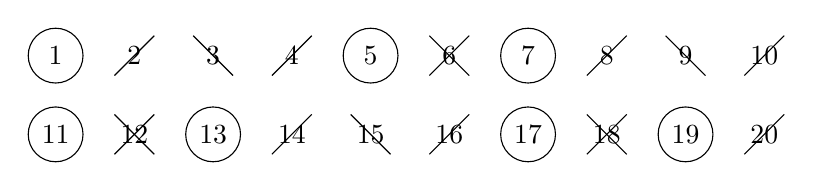
\begin{tikzpicture}
    \foreach \x in {1,...,10} {
      \coordinate (\x) at (\x,0);
    }
    \foreach \x in {11,...,20} {
      \coordinate (\x) at (\x-10,-1);
    }
    \foreach \x in {1,2,...,20} {
      \node at (\x) {\x};
    }
    \foreach \x in {2,4,...,20} {
      \node [strike out, draw=black, inner sep=7pt] at (\x) {};
    }
    \foreach \x in {3,6,...,20} {
      \node [strike out, draw=black, rotate=90, inner sep=7pt] at (\x) {};
    }
    \node [circle, draw=black, inner sep=7pt] at (1) {};
    \node [circle, draw=black, inner sep=7pt] at (5) {};
    \node [circle, draw=black, inner sep=7pt] at (7) {};
    \node [circle, draw=black, inner sep=7pt] at (11) {};
    \node [circle, draw=black, inner sep=7pt] at (13) {};
    \node [circle, draw=black, inner sep=7pt] at (17) {};
    \node [circle, draw=black, inner sep=7pt] at (19) {};
  \end{tikzpicture}
\end{center}
We are left with all the primes above 3, and 1. Alternatively, we can use the inclusion-exclusion principle to count how much is left.
Our interest is in using the sieve to count things: how many numbers are left?
\begin{align*}
  \hyperlink{def:pi}{\pi(20)} + 1 - \pi(\sqrt{20}) = 20 - \floor*{\frac{20}{2}} - \floor*{\frac{20}{3}} + \floor*{\frac{20}{6}}.
\end{align*}
This is the general idea: We get an expression relating some quantity we are interested in - the number of primes below a certain limit - in terms of how much we `sieved' out at each stage.
\subsection{Setup}
We generally use:
\begin{itemize}\hypertarget{def:sievesetup}
  \item a finite set $A \subset \mathbb{N}$ (the set to be sifted)
  \item a set of primes $P$ (the set of primes we sift out by, usually all primes).
  \item a sifting limit $z$ (sift with all primes in $P < z$)
  \item a sifting function
    \begin{equation*}
      S(A,P; z) = \sum_{n \in A} 1_{(n, P(z)) = 1}\nomenclature{$S(A,P;z)$}{sifting function}
    \end{equation*}
    where
    \begin{equation*}
      P(z) \coloneqq \prod_{\substack{p \in P \\ p < z}} p.
    \end{equation*}
    The goal is to estimate $S(A,P; z)$.
  \item For $d$, let
    \begin{equation*}
      A_d = \{n \in A : d \mid n\}.
    \end{equation*}
    We write
    \begin{equation*}
      |A_d| = \frac{f(d)}{d} X + R_d
    \end{equation*}
    where $f$ is completely multiplicative ($f(mn) = f(m) f(n)$ $\forall m,n$) and $0 \leq f(d)\; \forall d$.
    Note many textbooks write $\omega$ for $f$.
  \item Note that
    \begin{equation*}
      |A| = \frac{f(1)}{1} X + R_1 = X + R_1
    \end{equation*}
    so we think of $R_d$ as an error term
  \item We choose $f$ so that $f(p) = 0$ if $p \notin P$ (so $R_p = |A_p|$)
  \item Let
    \begin{equation*}
      W_P(z) \coloneqq \prod_{\substack{p < z \\ p \in P}} \left(1 - \frac{f(p)}{p}\right).
    \end{equation*}
\end{itemize}
\begin{eg}\leavevmode
  \begin{enumerate}[label=(\arabic*)]
    \item Take $\hyperlink{def:}{A} = (x, %)[
      x+y] \cap \mathbb{N}$, and $P$ the set of all primes, so
      \begin{align*}
        |A_d| &= \floor*{\frac{x+y}{d}} - \floor*{\frac{x}{d}} = \frac{x+y}{d} - \frac{x}{d} + \hyperlink{def:asymp}{\bigO(1)} \\
              &= \frac{y}{d} + \bigO(1)
      \end{align*}
      so $f(d) \equiv 1$ and $R_d = \bigO(1)$.
      So
      \begin{equation*}
        S(A,P;z) = \abs{\{x < n \leq x+y : \text{if }p \mid n\text{ then }p \geq z\}}
      \end{equation*}
      e.g.\ if $z \approx (x+y)^{\frac{1}{2}}$ then
      \begin{equation*}
        S(A,P; z) = \hyperlink{def:pi}{\pi(x+y)} - \pi(x) + \bigO((x+y)^{\frac{1}{2}})
      \end{equation*}
    \item Take
      \begin{equation*}A = \{1 \leq n \leq q : n \equiv a \pmod{q}\}.\end{equation*}
      Then
      \begin{equation*}A_d = \left\{1 \leq m \leq \frac{x}{d} : dm \equiv a \pmod{q}\right\}.\end{equation*}
      This congruence only has solutions if $(d,q) \mid a$, so
      \begin{align*}
        |A_d| &=
        \begin{cases}
          \frac{(d,q)}{dq} y + \bigO((d,q)) & \text{if } (d,q) \mid a \\
          \bigO((d,q)) & \text{otherwise}
        \end{cases} \\
        f(d) &=
        \begin{cases}
          (d,q) & \text{if } (d,q) \mid a \\
          0 & \text{otherwise}.
        \end{cases}
      \end{align*}
      We will do this example in more detail later, but it shows how $f$ can be more complicated, and that we can use sieve methods to count primes congruent to $a \pmod{q}$.
    \item What about twin primes? Take $A = \{n(n+2) : 1 \leq n \leq x\}$, and $P$ as all primes except $2$. So $p \mid n(n+2) \iff n \equiv 0 \text{ or } -2 \pmod{p}$. Now,
      \begin{align*}
        |A_p| = 2\frac{x}{p} + \bigO(1).
      \end{align*}
      So $f(p) = 2$, so $f(d) = 2^{\omega(d)}$.
      Then
      \begin{align*}
        S(A,P; x^{\frac{1}{2}}) &= \abs{\{1 \leq p \leq x : p, p+2 \text{ both prime}\}} + \bigO(x^{\frac{1}{2}}) \\
                                &= \pi_2(x) + \bigO(x^{\frac 12})
      \end{align*}
      We expect $\pi_2(x) \approx \frac{x}{(\log x)^2}$. We cannot prove the lower bound, but we can prove the upper bound using this sieve soon.
  \end{enumerate}
\end{eg}
\begin{nthm}[Sieve of Eratosthenes-Legendre]\label{thm:2.1}
  \begin{equation*}
    \hyperlink{def:sievesetup}{S(A,P; z)} = X W_p(z) + \bigO\left(\sum_{d \mid p(z)} R_d\right).
  \end{equation*}
\end{nthm}
\begin{proof}
  \begin{align*}
    S(A,P;z) &= \sum_{n \in A} 1_{(n, P(z)) = 1} \\
             &= \sum_{n \in A} \sum_{d \mid (n, P(z))}\hyperlink{def:mu}{ \mu(d)} \\
             &= \sum_{n \in A} \sum_{\substack{d \mid n \\ d \mid P(z)}} \mu(d) \\
             &= \sum_{d \mid P(z)} \mu(d) \sum_{n \in A} 1_{d \mid n} \\
             &= \sum_{d \mid P(z)} \mu(d) |A_d| \\
             &= X \sum_{d \mid P(z)} \frac{\mu(d) f(d)}{d} + \sum_{d \mid P(z)} \mu(d) R_d \\
             &= X \prod_{\substack{p \in P \\ p < z}} \left(1 - \frac{f(p)}{p}\right) + \hyperlink{def:asymp}{\bigO}\left(\sum_{d \mid P(z)} |R_d|\right). \qedhere
  \end{align*}
\end{proof}
\begin{ncor}\label{cor:2.2}
  \begin{equation*}
    \hyperlink{def:pi}{\pi(x+y)} - \pi(x) \hyperlink{def:asymp}{\ll} \frac{y}{\log \log y}.
  \end{equation*}
\end{ncor}
\begin{proof}
  In Example 1, recall $f \equiv 1$ and $|R_d| \hyperlink{def:asymp}{\ll} 1$, $X = y$.
  So
  \begin{align*}
    W_P(z) = \prod_{p \leq z} \left(1 - \frac 1p\right) \ll (\log z)^{-1}
  \end{align*}
  and
  \begin{equation*}
    \sum_{d \mid P(z)} |R_d| \ll \sum_{d \mid P(z)} 1 \leq 2^z.
  \end{equation*}
  So $\hyperlink{def:pi}{\pi(x+y)} - \pi(x) \ll \frac{y}{\log z} + 2^z \ll \frac{y}{\log \log y} $ by choosing $z = \log y$.
\end{proof}

\subsection{Selberg's sieve}
\newlec
From \nameref{thm:2.1}, we got
\begin{equation*}
  S(A,P;z) \leq XW + \bigO\left(\sum_{d \mid P(z)} |R_d|\right).
\end{equation*}
The problem here is that we have to consider $2^z$ many divisors of $P(z)$, so get $2^z$ many error terms.
We can do a different sieve, and only consider those divisors of $P(z)$ which are small, say $\leq D$.

The key part of \nameref{thm:2.1} was
\begin{equation*}
  1_{(n,P(z)) = 1} = \sum_{d \mid (n, P(z))} \mu(d).
\end{equation*}
For an upper bound, we note that it is enough to use \emph{any} function $F$ in place of $\mu$ such that
\begin{equation*}
  F(n) \geq
  \begin{cases}
    1 & n=1 \\
    0 & \text{otherwise}
  \end{cases}
\end{equation*}
(we used $F=\mu$ in the proof of \nameref*{thm:2.1})

Selberg's observation was that if $\lambda_i$ is an sequence of reals with $\lambda_1 = 1$ then
\begin{equation*}
  F(n) = \left(\sum_{d \mid n} \lambda_d\right)^2
\end{equation*}
works:
\begin{equation*}
  F(1) = \left(\sum_{d \mid 1} \lambda_d\right)^2 = \lambda_1^2 = 1.
\end{equation*}

We make the additional assumption on $f$ that $0 < f(p) < p$ if $p \in P$. Recall that $|A_p| = \frac{f(p)}{p} X + R_p$, so these are reasonable restrictions to have on a sieve.

This lets us define a new multiplicative function $g$ such that
\begin{equation*}
  g(p) = \left(1 - \frac{f(p)}{p}\right)^{-1} -1 = \frac{f(p)}{p - f(p)}
\end{equation*}
\begin{nthm}[Selberg's sieve]\label{thm:2.3}
  \begin{equation*}
    \forall t \quad S(A,P;z) \leq \frac{X}{G(t,z)} + \sum_{\substack{d \mid P(z) \\ d < t^2}} 3^{\omega(d)} |R_d|
  \end{equation*}
  where
  \begin{equation*}
    G(t,z) = \sum_{\substack{d \mid P(z) \\ d < t}} g(d).
  \end{equation*}
\end{nthm}
Recall
\begin{equation*}
  W = \prod_{\substack{p \in P \\ p \leq z}} \left(1 - \frac{f(p)}{p}\right)
\end{equation*}
so the expected size of $S(A,P;z)$ is $XW$. Note that as $t \to \infty$,
\begin{align*}
  G(t,z) &\to \sum_{d \mid P(z)} g(d) \\
         &= \prod_{p < z} (1 + g(p)) \\
         &= \prod_{p < z} \left(1 - \frac{f(p)}{p}\right)^{-1} = \frac{1}{W}.
\end{align*}

\begin{ncor}\label{cor:2.4}
  \begin{equation*}
    \hyperlink{def:pi}{\pi(x+y)} - \pi(x) \hyperlink{def:asymp}{\ll} \frac{y}{\log y}.
  \end{equation*}
\end{ncor}
Compare this with \cref{cor:2.2}.
\begin{proof}
  Take $A = \{x < n \leq x+y\}$, $f(p) = 1$, $R_d = \bigO(1)$, $X = y$.
  Since $g(p) = \frac{1}{p-1} = \frac{1}{\varphi(p)}$, so $g(d) = \frac{1}{\varphi(d)}$,
  The main term from \cref{thm:2.3} gives
  \begin{align*}
    G(z,z) &= \sum_{\substack{d \mid P(z) \\ d < z}} \prod_{p \mid d} (p-1)^{-1} \\
           &= \sum_{d = p_1 \dotsm p_r < z} \prod_i \sum_{k \geq 1}^\infty \frac{1}{p_i^k} \\
           &= \sum_{p < z} \sum_{\substack{k_r \geq 1 \\ p_1 \dotsm p_r < z}} \frac{1}{p_1^{k_1} \dotsm p_r^{k_r}} \\
           &= \sum_{n} \frac{1}{n} \text{ for $n$ where the square-free part of $n$ is $\leq t$}\\
           &\geq \sum_{d<z} \frac{1}{d} \\
           &\gg \log z.
  \end{align*}

  So the main term is $\ll \frac{y}{\log z}$.
  Note that $3^{\omega(d)} \leq \tau_3(d) \ll_\epsilon d^\epsilon$. So the error term is
  \begin{equation*}
    \ll_\epsilon t^\epsilon \sum_{d < t^2} 1 \ll t^{2 + \epsilon} = z^{2+\epsilon}
  \end{equation*}
  since we are taking $t = z$.
  So
  \begin{equation*}
    S(A,P;z) \ll \frac{y}{\log z} + z^{2+\epsilon} \ll \frac{y}{\log y}
  \end{equation*}
  by taking $z = y^{\frac{1}{3}}$.
\end{proof}

\begin{proof}[Proof of \cref{thm:2.3}]
  Let $(\lambda_i)$ be a sequence of reals, with $\lambda_1 = 1$, to be chosen later. Then
  \begin{align*}
    S(A,P;z) &= \sum_{n \in A} 1_{(n,P(z)) = 1} \\
             &\leq \sum_{n \in A} \left(\sum_{d \mid (n,P(z))} \lambda_d\right)^2 \\
             &= \sum_{d,e \mid P(z)} \lambda_d \lambda_e \sum_{n \in A} 1_{d \mid n,\ e \mid n} \\
             &= \sum_{d, e \mid P(z)} \lambda_d \lambda_e |A_{[d,e]}| \\
             &= X \sum_{d,e \mid P(z)} \lambda_d \lambda_e \frac{f([d,e])}{[d,e]} + \sum_{d,e \mid P(z)} \lambda_d \lambda_e R_{[d,e]}.
  \end{align*}
  $[d,e]$ denotes the least common multiple of $d$ and $e$. We will choose $\lambda_d$ such that $|\lambda_d| \leq 1$ and $\lambda_d = 0$ if $d \geq t$.
  Then
  \begin{align*}
    \abs{\sum_{d,e \mid P(z)} \lambda_d \lambda_e R_{[d,e]}} &\leq \sum_{\substack{d,e < t \\ d,e \mid P(z)}} |R_{[d,e]}| \\
                                                             &\leq \sum_{\substack{n \mid P(z) \\ n < t^2}} |R_n| \sum_{d,e} 1_{[d,e] = n}
  \end{align*}
  and
  \begin{equation*}
  \sum_{d,e} 1_{[d,e]=n} = 3^{\omega(n)}
  \end{equation*}
  as $n$ is squarefree.

  Let
  \begin{equation*}
    V = \sum_{d,e \mid P(z)} \lambda_d \lambda_e \frac{f([d,e])}{[d,e]}
  \end{equation*}
  Write $[d,e] = abc$ where $d = ab$, $e = bc$ and $(a,b) = (b,c) = (a,c) = 1$, which we can do since $\lambda_d=0$ if $d$ is not square-free.

\newlec
\begin{align*}
  V &= \sum_{c \mid P(z)} \frac{f(c)}{c} \sum_{\substack{ab \mid P(z) \\ (a,b) = 1}} \frac{f(a)f(b)}{ab} \lambda_{ac} \lambda_{bc} \\
    &= \sum_{c \mid P(z)} \frac{f(c)}{c} \sum_{\substack{ab \mid P(z)}} \frac{f(a)}{a} \frac{f(b)}{b} \sum_{d \mid a,\,d \mid b} \mu(d)\lambda_{ac} \lambda_{bc} \\
  &= \sum_{c \mid P(z)} \frac{f(c)}{c} \sum_{d \mid P(z)} \mu(d) \left(\sum_{d \mid a \mid P(z)} \frac{f(a)}{a} \lambda_{ac}\right)^2 \\
  \shortintertext{taking $ac=n$,}
  &= \sum_{d \mid P(z)} \mu(d) \sum_{c \mid P(z)} \frac{c}{f(c)} \left(\sum_{cd \mid n \mid P(z)} \frac{f(n)}{n} \lambda_n\right)^2 \\
  &= \sum_{d \mid P(z)} \mu(d) \sum_{c \mid P(z)} \frac{c}{f(c)} y_{cd}^2 \\
  &= \sum_{k \mid P(z)} \left(\sum_{cd = k} \mu(d) \frac{c}{f(c)}\right) y_k^2
\end{align*}
For primes $p$,
\begin{equation*}
  \sum_{cd = p} \mu(d) \frac{c}{f(c)} = -1 + \frac{p}{f(p)} = \frac{p-f(p)}{f(p)} = \frac{1}{g(p)}.
\end{equation*}
Therefore $\forall h \mid P(z)$
\begin{equation*}
  \sum_{cd=k} \mu(d) \frac{c}{f(c)} = \frac{1}{g(k)}.
\end{equation*}

Note that if $k \geq t$ then
\begin{equation*}
  y_k = \sum_{\substack{k \mid n \mid P(z)\\ h \geq t}} \frac{f(n)}{n} \lambda_n = 0
\end{equation*}
So
\begin{equation*}
  V = \sum_{\substack{k \mid P(z) \\ k < t}} \frac{y_k^2}{g(k)}
\end{equation*}
Want to choose $V$ as small as possible.

What is the relationship between $y_k$ and $\lambda_d$?
\begin{equation*}
  y_k = \sum_{k \mid n \mid P(z)} \frac{f(n)}{n} \lambda_n.
\end{equation*}
Fix $d$.
\begin{align*}
  \sum_{d \mid k \mid P(z)} \mu(k) y_k &= \sum_{h \mid P(z)} \mu(k) \sum_{n \mid P(z)} \frac{f(n)}{n} \lambda_n 1_{d \mid k} 1_{k \mid n} \\
                                       &= \sum_{n \mid P(z)} \frac{f(n)}{n} \lambda_{k} 1_{d \mid n} \sum_{d\ mid k \mid n} \mu(k)
\end{align*}
Considering this innermost sum, write $k = de$, so we have
\begin{equation*}
  \mu(d) \sum_{e \mid \frac{n}{d}} \mu(e) =
  \begin{cases}
    \mu(d) & n = d \\
    0 & n > d
  \end{cases}
\end{equation*}
Thus
\begin{align*}
  \sum_{d \mid k \mid P(z)} \mu(k) y_k = \mu(d) \frac{f(d)}{d} \lambda_d.
\end{align*}
Recall $\lambda_1=1$, so must have
\begin{equation*}1 = \sum_{k \mid P(z)} \mu(k) y_k\end{equation*}
\begin{align*}
  1 = \left(\sum_{\substack{k \mid P(z) \\ k < t}} \mu(k) y_k g(k)^{\frac 12} \times \frac{1}{g(k)^{\frac 12}}\right)^2 \leq \left(\sum_{\substack{k \mid P(z) \\ k<t} g(k)}\right) \left(\sum_{\substack{k \mid P(z) \\ k < t}} \frac{y_k^2}{g(k)}\right) = GV
\end{align*}
So $V \geq \frac{1}{G}$; but equality holds iff $\exists c$ such that $\forall k$,
\begin{align*}
  \frac{\mu(k) y_k}{g(k)^{\frac{1}{2}}} = c g(k)^{\frac 12} \\
  \implies y_k = c \mu(k) g(k) \quad (k < t)
\end{align*}

What is $c$? We know that
\begin{equation*}
  1 = c \sum_{\substack{k \mid P(z)}} \mu(k)^2 g(k) = cG
\end{equation*}
so choose $c = \frac{1}{G}$. Check:
\begin{enumerate}
  \item $\lambda_1 = 1$ \checkmark
  \item $\lambda_d = 0$ if $d \geq t$ \checkmark
  \item $|\lambda_d| \leq 1$:
    \begin{equation*}
      \lambda_d = \mu(d) \frac{d}{f(d)} \sum_{d \mid k \mid P(z)} \mu(k) y_k
    \end{equation*}
    so
    \begin{align*}
      |\lambda_d| = \frac{d}{f(d)} \frac{1}{G} \sum_{d \mid k \mid P(z)} g(k).
    \end{align*}

    \begin{align*}
      G &= \sum_{\substack{e \mid P(z) \\ e<t}} g(e) \\
        &= \sum_{k \mid d} \sum_{\substack{e \mid P(z) \\ e < t \\ (d,e)=k}} g(e) \\
        &= \sum_{k \mid d} \sum_{\substack{n \mid P(z) \\ (m,d) = 1 \\ m < \frac{t}{k}}} g(m) \\
        &\geq \left(\sum_{k \mid d} g(k)\right) \left(\sum_{\substack{m \mid P(z) \\ (m,d) = 1 \\ m < \frac{t}{d}}} g(m)\right)
    \end{align*}

    Note that for primes $p$,
    \begin{equation*}
      \sum_{k \mid p} g(k) = 1 + \frac{f(p)}{p - f(p)} = \frac{p}{p - f(p)} = \frac{p}{f(p)} g(p).
    \end{equation*}
    So
    \begin{align*}
      G \geq \frac{d}{f(d)} g(d) \left(\sum_{\substack{m \mid P(z) \\ (m,d) = 1 \\ m < \frac{t}{d}}} g(m)\right) = \frac{d}{f(d)} \sum_{d \mid k \mid P(z)} g(k) = |\lambda_d| G
    \end{align*}
  so $|\lambda_d| \leq 1$. \qedhere
\end{enumerate}
\end{proof}
\begin{nthm}[Brun]\label{thm:2.5}
  Let $\pi_2(x) = \# \{1 \leq n \leq n : n \text{ and } n+2 \text{ are prime}\}$.
  Then
  \begin{align*}
    \pi_2(x) \ll \frac{x}{(\log x)^2}
  \end{align*}
\end{nthm}
We can reasonably expect $\pi_2(x) \asymp \frac{x}{(\log x)^2}$, but proving the lower bound would mean there are infinitely many twin primes.
\begin{proof}
  Take $A = \{n(n+2) : 1 \leq n \leq x\}$, and $P=$ all primes except 2.
  Then
  \begin{align*}
    |A_d| = \#\{1 \leq n \leq x : d \mid n(n+2)\}
  \end{align*}
  if $d = p_1 \dotsm p_r$ odd and squarefree.
  \begin{align*}
    d \mid n(n+2) \iff p_i \mid n(n+2) \ \forall i \iff n \equiv 0 \text{ or} -2 \pmod{p_i} \ \forall i
  \end{align*}
  By CRT, true iff $n$ lies in one of $2^{\omega(d)}$ many residue classes mod $d$. So
  \begin{align*}
    |A_d| = \frac{2^{\omega(d)}}{d} x + \bigO(2^{\omega(d)})
  \end{align*}
  so $f(d) = 2^{\omega(d)}$ for $d$ odd, square-free, and $R_d \ll 2^{\omega(d)}$.

  By Selberg's sieve, with $t = z = x^{\frac{1}{4}}$,
  \begin{align*}
    \pi_2(x) &\leq \# \{1 \leq n \leq x : p \mid n(n+2) \Rightarrow p = 2 \text{ or } p > x^{\frac 14}\} + \bigO(x^{\frac{1}4}) \\
             &= S(A,P; x^{\frac{1}{4}}) + \bigO(x^{\frac 14}) \\
             &\leq \frac{x}{G(z,z)} + \bigO(\sum_{\substack{d \mid P(z) \\ d < z^2}} 6^{\omega(d)})
  \end{align*}
  Focus on the error term first:
  \begin{align*}
    \sum_{d < z^2} 6^{\omega(d)} \leq z^{2 + o(1)} = x^{\frac{1}{2} + o(1)}.
  \end{align*}

\end{proof}
\clearpage
\printnomenclature
\printindex
\end{document}
